\documentclass{article}
\usepackage[utf8]{inputenc}
\usepackage{graphicx}
\usepackage{wrapfig}
\usepackage{array}
\usepackage{siunitx}
\usepackage{xcolor}
\usepackage{multicol}
\usepackage{amssymb}
\setlength{\columnseprule}{1pt}

\title{Steady State Response of	RLC	Circuits \\ Lab Report 4 \\ ELP100}
\author{Yash Agarwal \\ 2021EE10638 \\ Group 29}
\date{May 16, 2022}

\begin{document}
\pagecolor{yellow!15}
\maketitle
\vspace{15px}
\tableofcontents
\newcolumntype{V}{>{\centering\arraybackslash} m{.4\linewidth} }
\newpage
\section{Steady State Response in RLC Circuit}
\subsection{Aim}
To draw the phasor diagram of series RLC circuit and compare the experimental and theoretical results.
\subsection{Apparatus}
\begin{enumerate}
\item Breadboard and Jumpers
\item Multimeter
\item Capacitor, Resistor, Inductor
\item Digital Storage Oscilloscope (DSO1052B)
\item Function Generator (0 – 3 MHz)
\end{enumerate}

\subsection{Theory}
\vspace{5px}
\subsubsection{Phase of a AC Wave}
\begin{wrapfigure}{R}{0.35\textwidth}
\fcolorbox{black}{white}{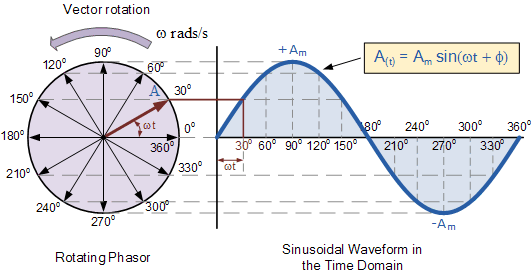
\includegraphics[width=0.35\textwidth]{accircuits-acp25.png}}
\end{wrapfigure}
Sinusoidal signals are characterized by their amplitude, their frequency and their phase. In many circuits the frequency is fixed (perhaps at the frequency of the AC supply) and we are interested in only amplitude and phase. In such cases, we often use phasor diagrams which represent amplitude and phase within a single diagram. Phasor diagrams can be used to represent the addition of signals.


\subsubsection{Phasor of a Real Inductor}
\begin{wrapfigure}{R}{0.2\textwidth}
\fcolorbox{black}{white}{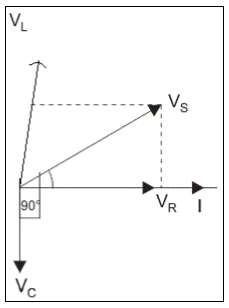
\includegraphics[width=0.2\textwidth]{Phasor.png}}
\end{wrapfigure}
In real life, actually there is not a pure inductor because of the wire present in it and this winding wire has some resistance. Hence the practical inductor is not a pure inductance represented by a \ang{90} phase angle and thus $V_L$ is at an angle slightly less than \ang{90} in phasor diagram.

\noindent
\[The \ Angle \ between \ V_L and \ V_R \ is \ tan^{-1}\frac{X_L}{r}\]
\[The \ Impedance \ in \ RLC\ Circuit\ is \ Z=R+(X_L- X_C)j\]

\subsection{Breadboard Setup}
\vspace{5px}

\begin{center}
\fcolorbox{black}{white}{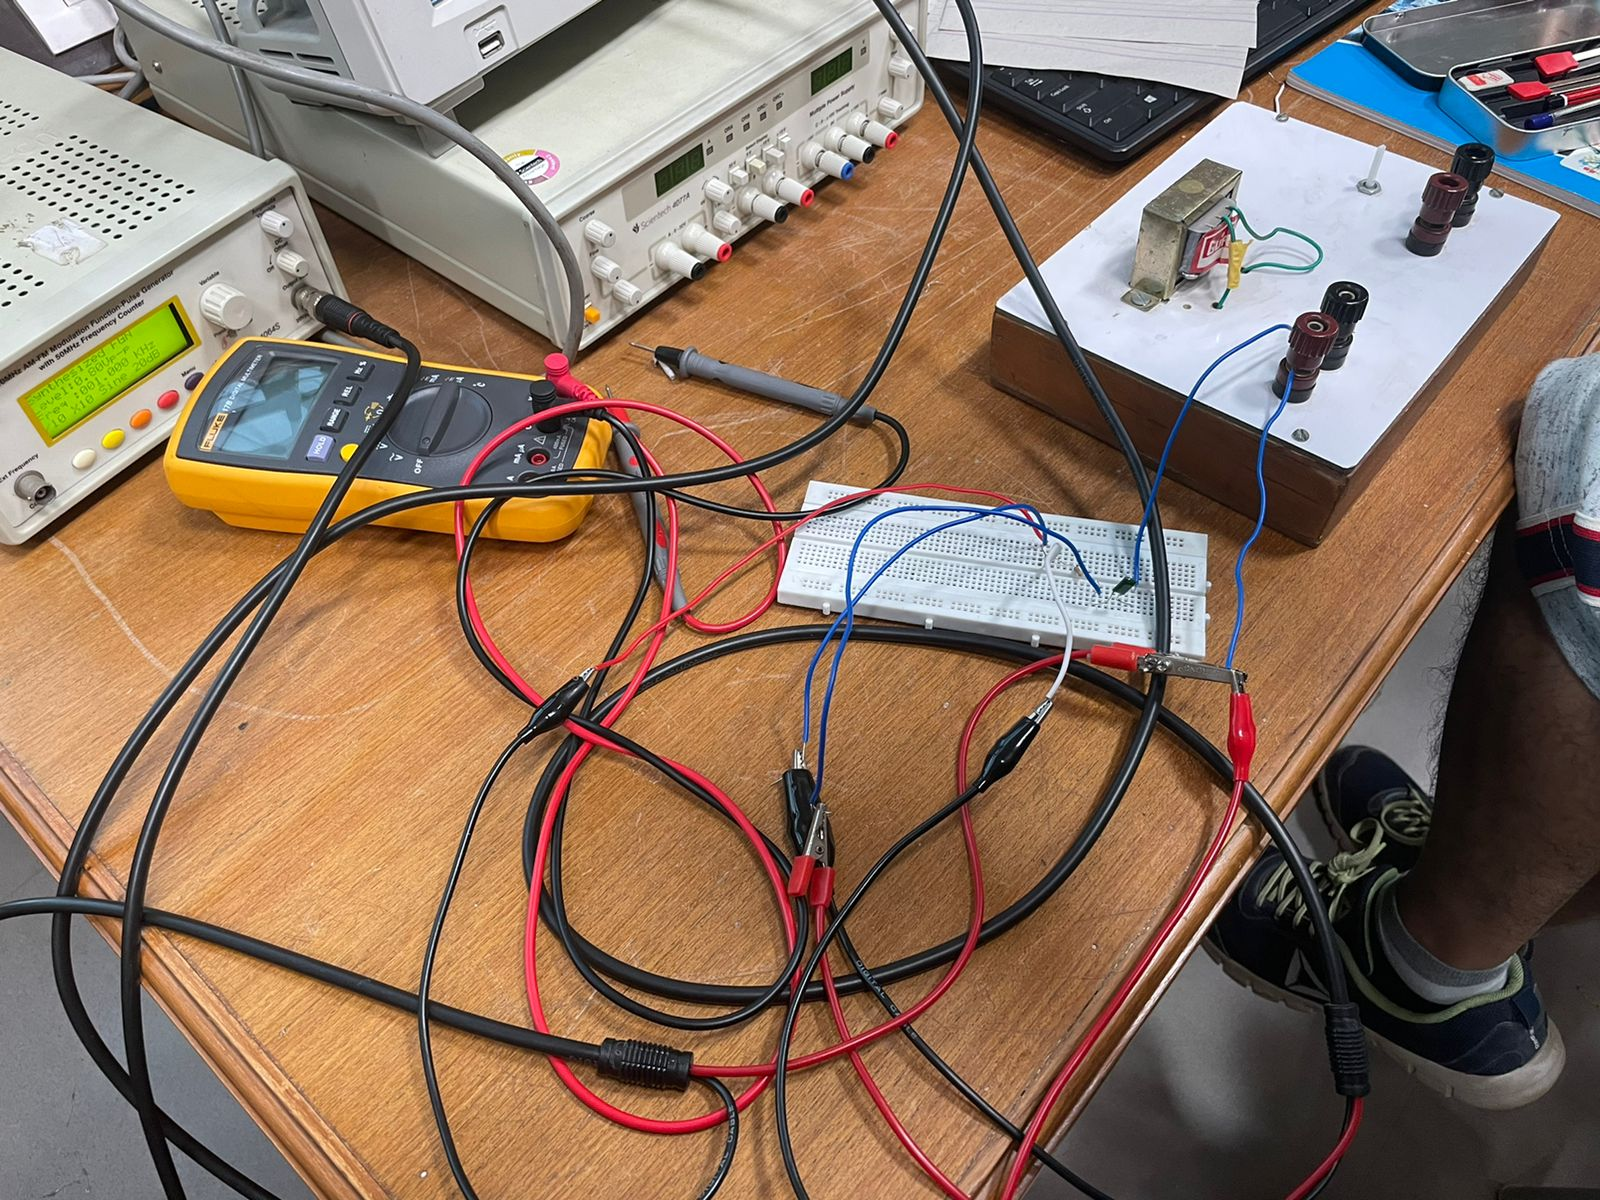
\includegraphics[width=0.9\columnwidth, height=150px]{Circuit.jpeg}} \\ \vspace{5px}
Circuit with $R=1 k\Omega$, $L=2H$, $C= 0.01 \mu F$ and $V_{PP}=2V$ \\
\end{center}

\subsection{Images of DSO}
\vspace{5px}
\begin{multicols}{2}
\begin{center}
\fcolorbox{black}{white}{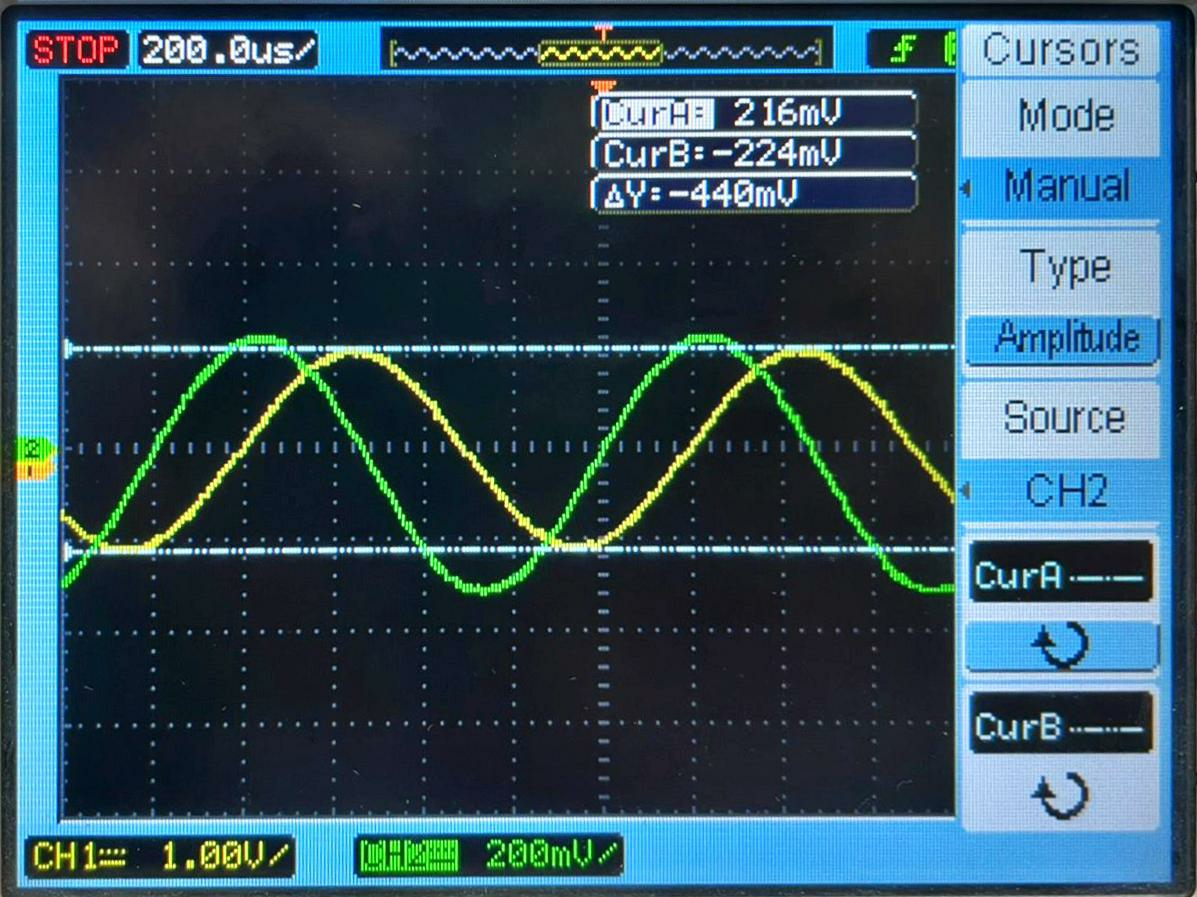
\includegraphics[width=0.9\columnwidth, height=110px]{VC.jpeg}} \\ \vspace{5px}
Voltage across Capacitor\\

\columnbreak

\fcolorbox{black}{white}{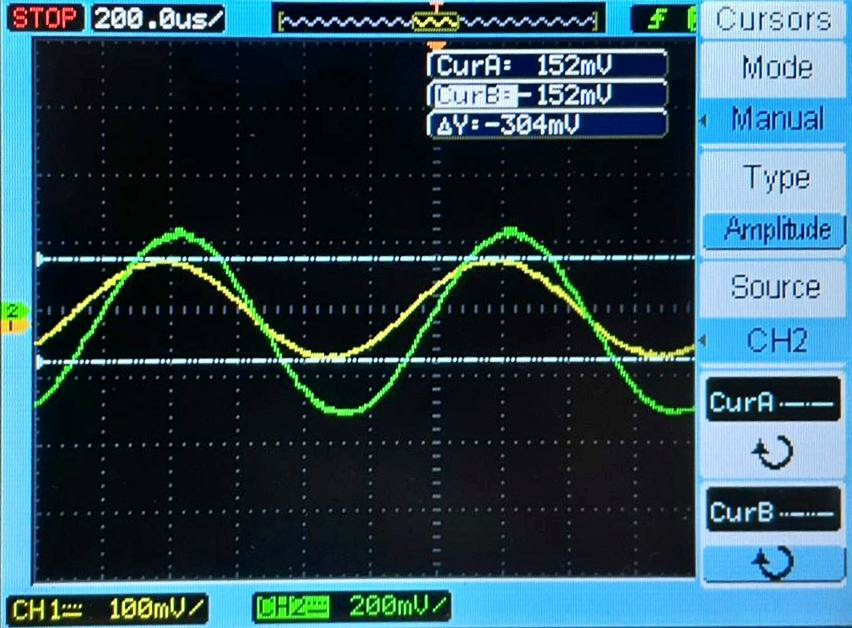
\includegraphics[width=0.9\columnwidth, height=110px]{VR.jpeg}} \\ \vspace{5px}
Voltage across Resistor
\end{center}
\end{multicols}
\begin{multicols}{2}
\begin{center}
\fcolorbox{black}{white}{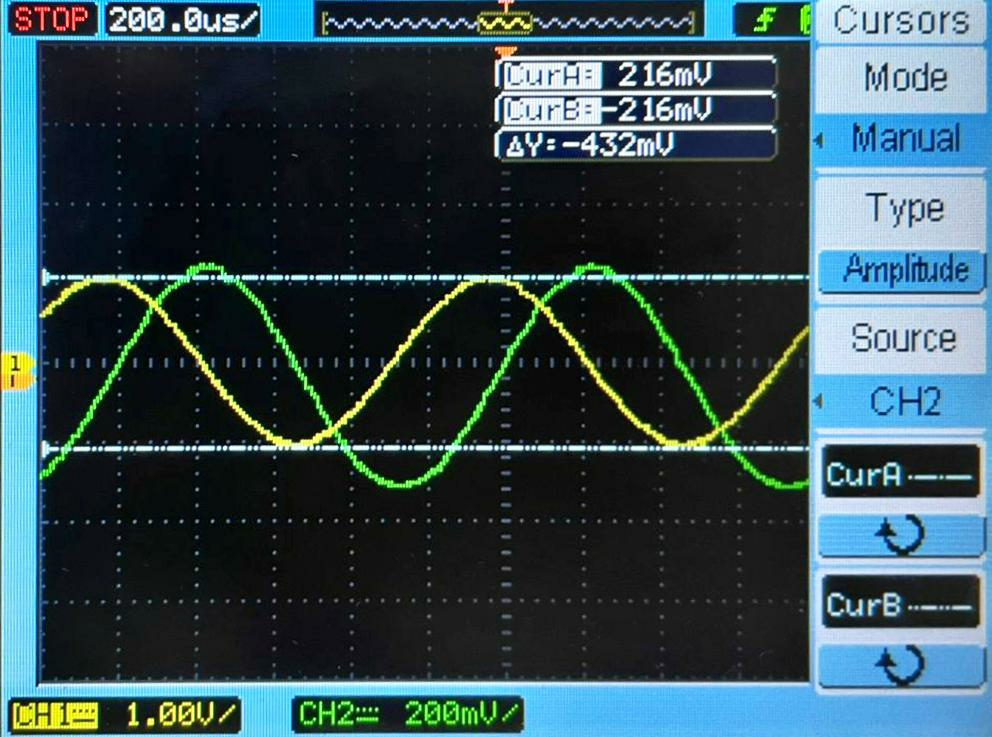
\includegraphics[width=0.9\columnwidth, height=110px]{VLr.jpeg}} \\ \vspace{5px}
Voltage across Real Inductor \\

\columnbreak

\fcolorbox{black}{white}{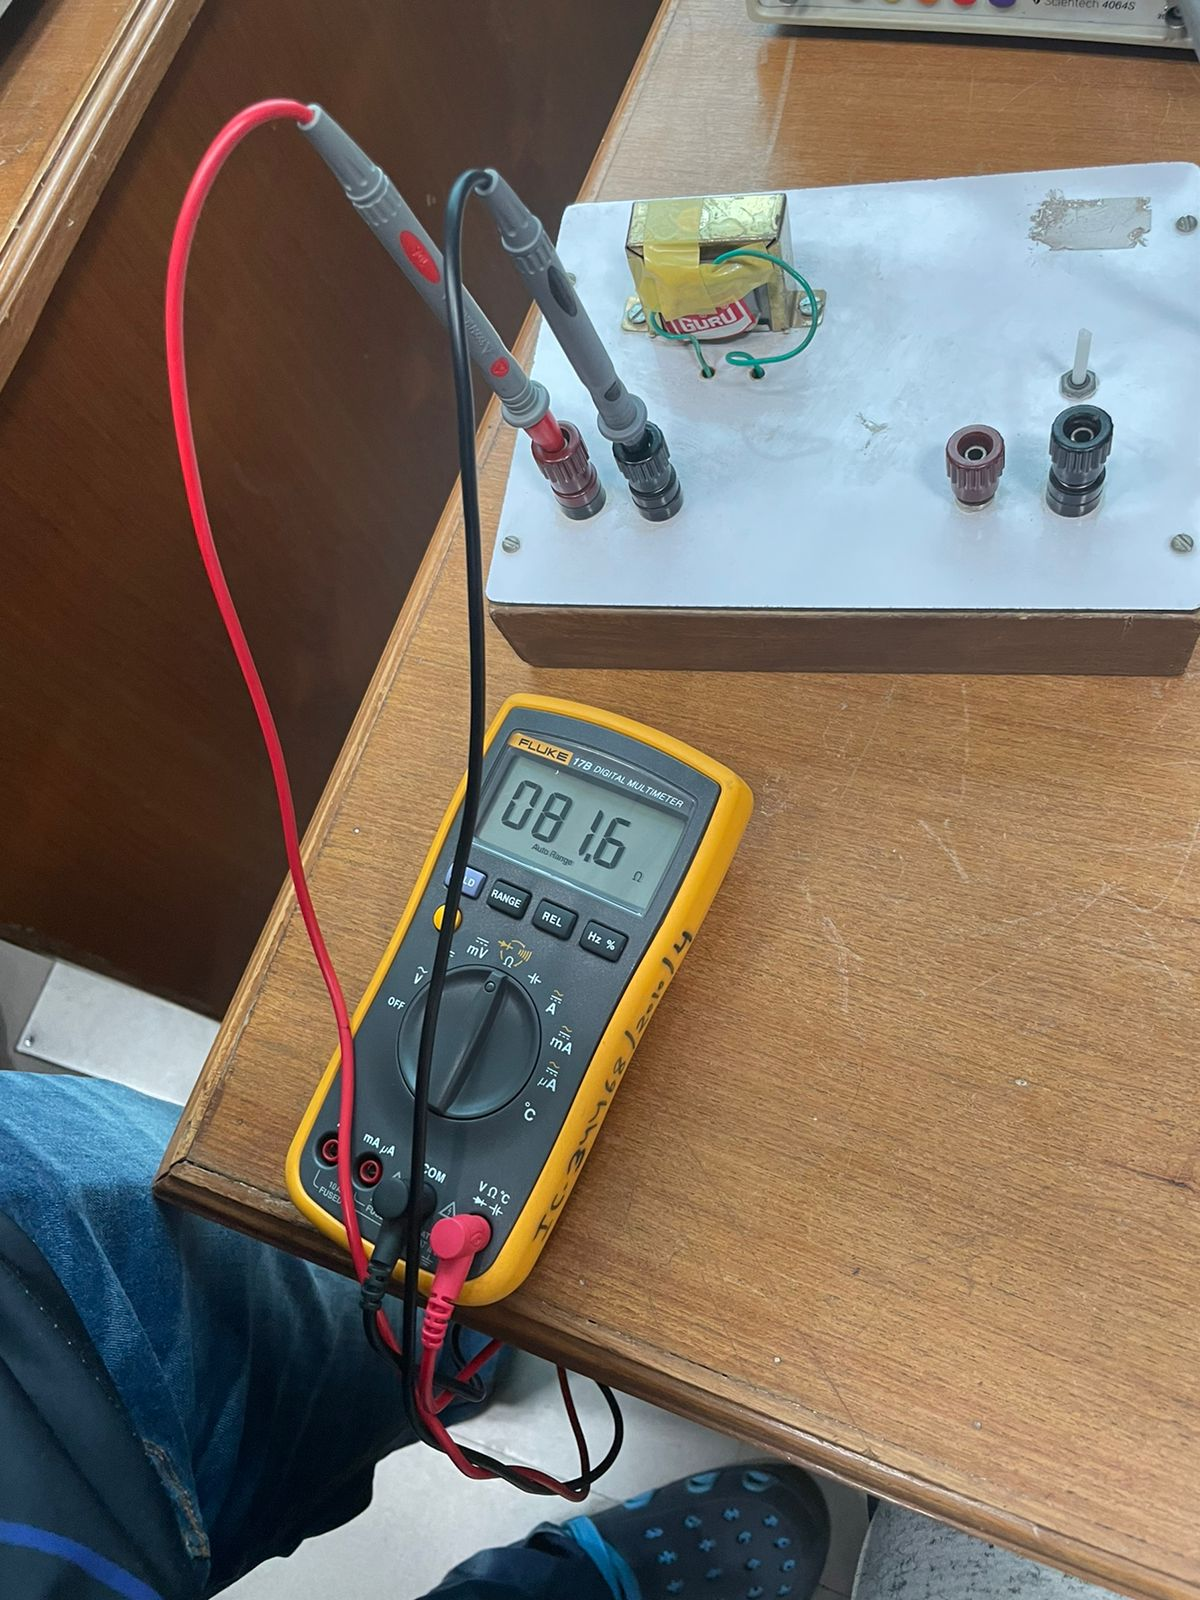
\includegraphics[width=0.9\columnwidth, height=110px]{Lr.jpeg}} \\ \vspace{5px}
Measurement of Resistance of Inductor
\end{center}
\end{multicols}
\newpage
\subsection{Observation}
\vspace{5px}
\begin{center}
\begin{tabular}{| c | c | c | c | c | c |} 
 \hline
    \ & \ & \ & \ & \ & \ \\
    Frequency & $V_0$ & $V_R$ & $V_C$ & $V_L$ & $i=\frac{V_R}{R}$\\ [1em]
    \hline
    \ & \ & \ & \ & \ & \ \\
    1kHz & 2V & 0.304V & 0.44V & 0.432V & 0.304mA \\
    2kHz & 2.1V & 0.205V & 1.47V & 3.22V & 0.207mA \\
    \ & \ & \ & \ & \ & \ \\
 \hline
\end{tabular}
\end{center}

\subsection{Calculation}
\vspace{5px}
\begin{center}
\begin{tabular}{| c | c | c | c |} 
 \hline
    \ & \ & \ & \ \\
    Frequency & $V_L$ & $X_L=2\pi Lf$ & Phase Difference \\ [1em]
    \hline
    \ & \ & \ & \ \\
    1kHz & 0.432V & 12566.37 & \ang{89.62} \\
    2kHz & 3.22V & 25132.74 & \ang{89.81} \\
    \ & \ & \ & \ \\
 \hline
\end{tabular}
\end{center}
\vspace{5px}
\begin{center}
\begin{tabular}{| c | c | c | c |} 
 \hline
    \ & \ & \ & \ \\
    $V_L$ & i & Phase Difference & r \\ [1em]
    \hline
    \ & \ & \ & \ \\
    0.432V & 0.304mA & \ang{89.62} &  $74.37\Omega$\\
    3.22V & 0.207mA & \ang{89.81} &  $58.32\Omega$\\
    \ & \ & \ & \ \\
 \hline
\end{tabular}
\end{center}
The error is expected due to mismatch of resistance values of the original circuit with the expected values, so the inductance coil’s resistance comes out to be nearly proportionally smaller.

\subsection{Phasors}
\begin{multicols}{2}
\begin{center}
\fcolorbox{black}{white}{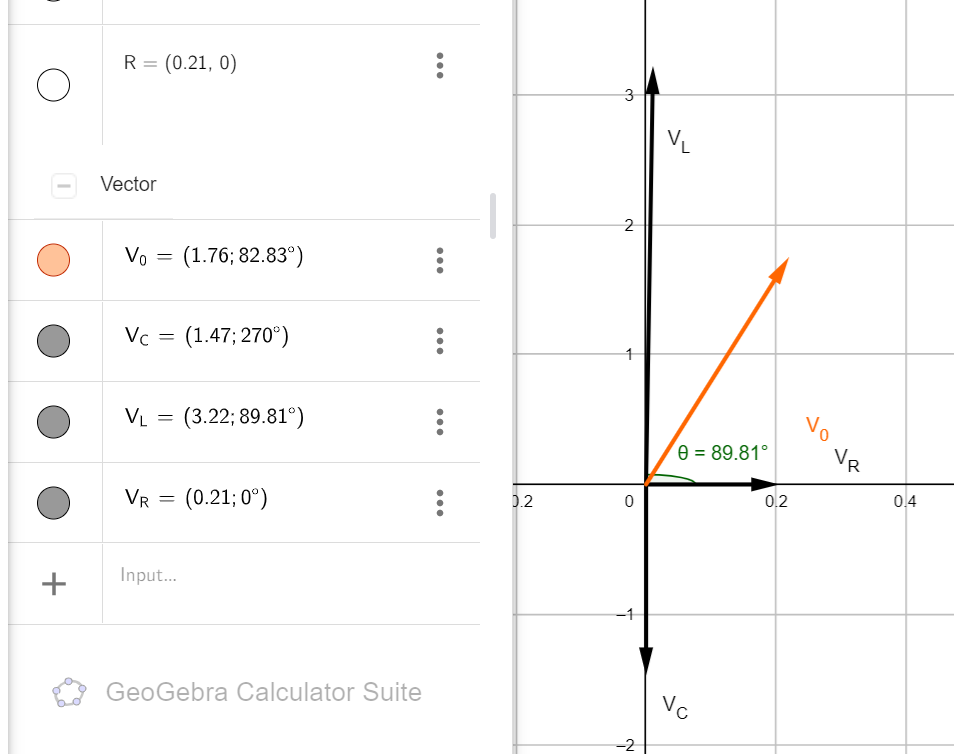
\includegraphics[width=0.9\columnwidth, height=110px]{Screenshot 2022-05-19 004703.png}} \\ \vspace{5px}
Phasor for $1^{st}$ Observation  \\

\columnbreak

\fcolorbox{black}{white}{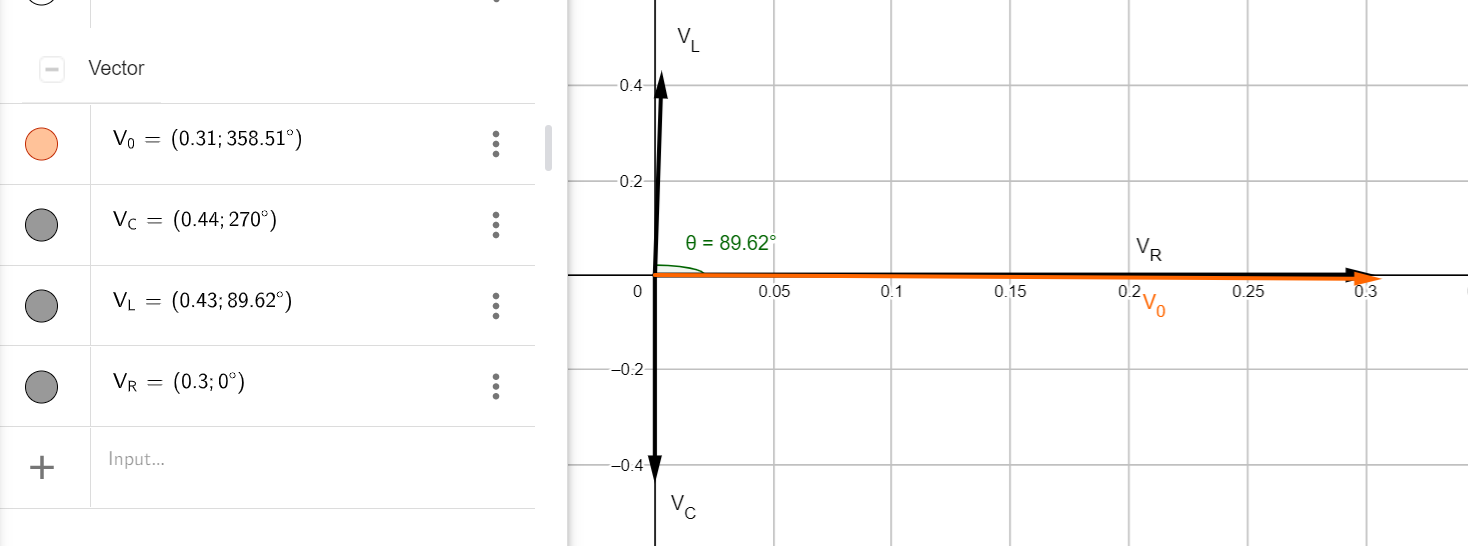
\includegraphics[width=0.9\columnwidth, height=110px]{Screenshot 2022-05-19 004506.png}} \\ \vspace{5px}
Phasor for $2^{nd}$ Observation
\end{center}
\end{multicols}

\subsection{Conclusion}
The variation in the reading may be due to some finite resistance in the connecting wires. Moreover, due to deflection in the reading of the multimeter, the values obtained might not be exact, as the error in the values are acceptable till they are not more than the Least Count.

\vspace{10px}
\section{Sources of Error}
\begin{itemize}
\item Scale of multi-meter not appropriate for measurements
\item Loose Connections
\item Resistance of wires not taken into account, and also giving rise to inconsistency due to increase in resistance due to heating
\item Change in the connections while circuit is closed.

\end{itemize}

\vspace{5px}

\section{Precautions}

\begin{itemize}
\item Make the connections neat and tight
\item Don’t leave the switch on for long continuous periods of time.
\item Wear proper shoes and use insulated tools
\end{itemize}

\vspace{5px}

\section{Concluding Remarks}
We evaluated the steady state response of a series RLC circuit to an ac input in the above experiment, and we analysed it by producing phasor diagrams and validating the impedance relationships with the measured values. We also confirmed that the phase difference between voltage signals across a resistor and a capacitor is a right angle, as is the phase difference between an inductor and a resistor (the reason for this is that the inductor coil is not ideal and hence has some finite non zero resistance).
\end{document}
